\section{Fractional Differential Equations (FDEs)}
Differential equations involving fractional differential operators
have recently proved to be valuable tools in the modeling of many
physical phenomena.

We will focus our analysis in this section on FDEs of the Caputo type of the form
\begin{equation}
    \leftindex[I]^C {D^{\alpha}} y(t) = f(t,y(t))
\end{equation}
And some parts will deal with a slightly more general class of problems
then we will look into some of the methods to solve linear and nonlinear FDEs

The reason why we will use the Caputo derivative that RL fractional derivative $D^\alpha$ 
in order to obtain a particular solution to the straightforward form of a FDE
\[
    D^\alpha y(t) = f(t,y(t))
\]
We need to specify $m$ initial conditions corresponding to it and it must be of the form
\[
    \left[D^{\alpha-k} y(t)\right]_{t=0} = \beta_k \quad,\quad k = 1,2,\dots,m
\]
With given values $\beta_k$. Thus we are forced to specify some fractional derivatives
of the function $y$. In practical applications, these values are frequently
not available, and it may not even be clear what their physical meaning is

Therefore Caputo has suggested that one should incorporate the classical derivatives 
(of integer order) of the function $y$, as they are commonly used in initial value problems 
with integer order equations, into the fractional order equation, using the relation between RL and Caputo derivatives
\[
    \leftindex[I]^C {D^{\alpha}} y(t) = D^\alpha (y-T_{m-1}[y])
\]
Where $T_{m-1}[y]$ is the Taylor polynomial of order $m-1$ for $y$, centered at
$0$. Then, one can specify the initial conditions in the classical form
\[
    y^{(k)}(0) = \beta_k \quad,\quad k=0,1,2,\dots,m-1 
\]

In the classical theory of integer order ordinary differential equations, it is well
known that unique solutions can only be expected if the differential equation is accompanied by certain additional conditions. 
The same observation is true in the fractional case. The question is then where on the $t-axis$ such condition(s) should be imposed.

By choosing the differential operator starting point, that is, the point $0$ we have answered this question. 
Interpreting the free variable $t$ as a time variable,
this amounts to providing information at the beginning of the process that the
differential equation describes and to seeking the process behavior for times that are
in the future of this instant.

\subsection{Initial Value Problems For Single Term Equations}
We will study IVPs in the form (6.1)
Since exactly one differential operator occurs in this equation, this type of
equations is known as a single term FDE.

Thus the IVP will be in the form 
\begin{equation}
    \begin{cases}
        \leftindex[I]^C {D^{\alpha}} y(t) = f(t,y(t))
        \\
        I.C \Longrightarrow y^{(k)}(0) = \beta_k \quad,\quad k=0,1,2,\dots,m-1 
    \end{cases}
\end{equation}
We can Consider the classical theory as a special case. 
Many (but not all) classical results (and their proofs) can be generalized to this fractional setting

% Almost all results are formulated for $d$-dimensional systems of equations 
% with arbitrary $d \in \mathbb{N}$, that is, we assume the function $y(t)$ is vector valid function map an
% interval $[0, T]$ to $\mathbb{R}^d$. Consequently, the initial values $\beta_k$ are vectors in $\mathbb{R}^d$, and the
% function $f$ is assumed to map a subset of $[0, T]\times\mathbb{R}^d$ to $\mathbb{R}^d$.

\subsubsection{Existence And Uniqueness Of Solutions}
The most important results in the classical theory, Peano's existence theorem and the
Picard-Lindelöf uniqueness theorem, remain valid in the fractional setting too but with some more conditions. Their
proofs are based on an equivalence between the IVP and a Volterra integral equation. 

Consider the IVP (6.2) let $f$ be a Continuous function if we apply $I^\alpha$ for both sides we get 
\begin{align*}
    \leftindex[I]^C {D^{\alpha}} y(t) &= f(t,y(t))
    \\
    y(t) - \sum_{k=0}^{m-1} \frac{t^k}{k!} y^{(k)}(0) &= I^\alpha f(t,y(t))
\end{align*}
Now we will state and proof the Theorem that makes function $y(t) \in C[0, T]$ a solution of
this nonlinear Volterra integral equation of the second kind
\begin{equation}
    y(t) = \sum_{k=0}^{m-1} \frac{t^k}{k!} y^{(k)}(0) + \frac{1}{\Gamma(\alpha)} \int_{0}^{t} (t-s)^{\alpha-1}f(s,y(s)) \hquad ds
\end{equation}
And then we will state the conditions that makes the equation (6.3) equivalent to the IVP (6.2)

BUT first let's build some definitions that we will use in our proof 
\vmasafa
\begin{definition}[Complete Space]
    The metric space $X$ is said to be Complete if every Cauchy sequence in $X$ 
    converges to a limit point in $X$
\end{definition}
\vmasafa
\begin{definition}[Banach Space]
    A Banach Space is a complete normed space 
    \\
    Examples : $\mathbb{R}^n , \mathbb{C}^n , C[a,b]$ are Banach
\end{definition}

\begin{lemma}
    A closed subspace of a Banach space is a Banach space
\end{lemma}
\begin{proof}[Proof]
    Let $X$ be a Banach Space then it is Complete 
    
    \begin{adjustwidth}{1cm}{2cm}
        $\therefore$ Every Cauchy sequence in $X$ converges to a limit point in $X$ 
    
        $\therefore$ $X$ is Closed and bounded
    
        Now let $E$ be Closed subspace of $X$ 
    
        $\therefore$ It is bounded with the same boundaries of $X$
    
        $\therefore$ $E$ is closed and bounded $\implies$ it contains all it's limit point 
    
        $\therefore$ Every Cauchy sequence in $E$ converges to a limit point in $E$ then $E$ is Complete normed space then it is Banach
    \end{adjustwidth}
\end{proof}
\vmasafa
\begin{definition}[Continuous Operator]
    An operator $T$ is said to be continuous at a point $x_0$ if 
    \[
        \forall \epsilon>0 , \exists \delta>0 \text{ such that } ||x-x_0|| \implies ||Tx-Tx_0|| < \epsilon
    \]
    $T$ is continuous on $X$ if $T$ is continuous at every point, $x \in X$

    Let $T : X \to Y$ be a linear operator then 
    \begin{enumerate}
        \item $T$ is continuous if and only if , $T$ is bounded
        \item If $T$ is continuous at a point then it's continuous
    \end{enumerate}
\end{definition}
% \vmasafa
% \begin{definition}[Compact Metric Space]
%     A metric space $X$ is said to be compact if every sequance in $X$ has a convergent subsequance in $X$
% \end{definition}

\newpage
\begin{definition}[Convex Set]
    A subset $A$ of $X$ is said to be Convex if for $x,y \in A$ we have 
    \[
        M := \left\{ z \in X : z = \alpha x + (1-\alpha)y \quad,\quad 0 \leq \alpha \leq 1 \right\} \subset A
    \]
    $M$ is called a closed segment with boundary points $x,y$
    \begin{center}
    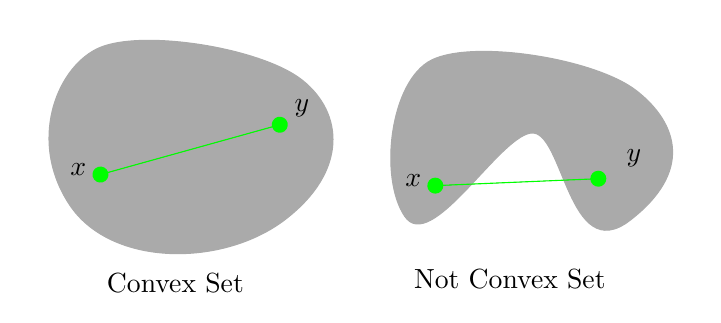
\begin{tikzpicture}[x=0.75pt,y=0.75pt,yscale=-1,xscale=1]
        %uncomment if require: \path (0,300); %set diagram left start at 0, and has height of 300
        
        %Shape: Polygon Curved [id:ds2968865898515556] 
        \draw  [color={rgb, 255:red, 170; green, 170; blue, 170 }  ,draw opacity=1 ][fill={rgb, 255:red, 170; green, 170; blue, 170 }  ,fill opacity=1 ] (153,42.83) .. controls (173,32.83) and (232,42) .. (252,57.83) .. controls (272,73.67) and (274,101.67) .. (244,124.83) .. controls (214,148) and (160,148) .. (140,118) .. controls (120,88) and (133,52.83) .. (153,42.83) -- cycle ;
        %Straight Lines [id:da27627405204315614] 
        \draw [color={rgb, 255:red, 0; green, 255; blue, 0 }  ,draw opacity=1 ][fill={rgb, 255:red, 0; green, 0; blue, 0 }  ,fill opacity=1 ]   (154.8,103.33) -- (241.2,79.33) ;
        \draw [shift={(241.2,79.33)}, rotate = 344.48] [color={rgb, 255:red, 0; green, 255; blue, 0 }  ,draw opacity=1 ][fill={rgb, 255:red, 0; green, 255; blue, 0 }  ,fill opacity=1 ][line width=0.75]      (0, 0) circle [x radius= 3.35, y radius= 3.35]   ;
        \draw [shift={(154.8,103.33)}, rotate = 344.48] [color={rgb, 255:red, 0; green, 255; blue, 0 }  ,draw opacity=1 ][fill={rgb, 255:red, 0; green, 255; blue, 0 }  ,fill opacity=1 ][line width=0.75]      (0, 0) circle [x radius= 3.35, y radius= 3.35]   ;
        %Shape: Polygon Curved [id:ds906687188537532] 
        \draw  [color={rgb, 255:red, 170; green, 170; blue, 170 }  ,draw opacity=1 ][fill={rgb, 255:red, 170; green, 170; blue, 170 }  ,fill opacity=1 ] (314.33,48.17) .. controls (334.33,38.17) and (393.33,47.33) .. (413.33,63.17) .. controls (433.33,79) and (440,102.17) .. (410,125.33) .. controls (380,148.5) and (377.84,80.69) .. (362,83.33) .. controls (346.16,85.97) and (313.8,142.03) .. (301.33,123.33) .. controls (288.87,104.64) and (294.33,58.17) .. (314.33,48.17) -- cycle ;
        %Straight Lines [id:da8771843126448762] 
        \draw [color={rgb, 255:red, 0; green, 255; blue, 0 }  ,draw opacity=1 ][fill={rgb, 255:red, 0; green, 0; blue, 0 }  ,fill opacity=1 ]   (316.13,108.67) -- (394.67,105.33) ;
        \draw [shift={(394.67,105.33)}, rotate = 357.57] [color={rgb, 255:red, 0; green, 255; blue, 0 }  ,draw opacity=1 ][fill={rgb, 255:red, 0; green, 255; blue, 0 }  ,fill opacity=1 ][line width=0.75]      (0, 0) circle [x radius= 3.35, y radius= 3.35]   ;
        \draw [shift={(316.13,108.67)}, rotate = 357.57] [color={rgb, 255:red, 0; green, 255; blue, 0 }  ,draw opacity=1 ][fill={rgb, 255:red, 0; green, 255; blue, 0 }  ,fill opacity=1 ][line width=0.75]      (0, 0) circle [x radius= 3.35, y radius= 3.35]   ;
        
        % Text Node
        \draw (139.07,96.73) node [anchor=north west][inner sep=0.75pt]    {$x$};
        % Text Node
        \draw (247.07,66.13) node [anchor=north west][inner sep=0.75pt]  [color={rgb, 255:red, 0; green, 0; blue, 0 }  ,opacity=1 ]  {$y$};
        % Text Node
        \draw (300.4,102.07) node [anchor=north west][inner sep=0.75pt]    {$x$};
        % Text Node
        \draw (407.07,90.13) node [anchor=north west][inner sep=0.75pt]  [color={rgb, 255:red, 0; green, 0; blue, 0 }  ,opacity=1 ]  {$y$};
        % Text Node
        \draw (156.67,150) node [anchor=north west][inner sep=0.75pt]   [align=left] {Convex Set};
        % Text Node
        \draw (304.67,148) node [anchor=north west][inner sep=0.75pt]   [align=left] {Not Convex Set};
        \end{tikzpicture}
    \end{center}
\end{definition}
\begin{lemma}[]
    A ball in a normed Space is Convex
\end{lemma}
\begin{proof}[Proof]
    Let $x,y$ be two points in a ball $B(a,r) \implies ||x-a|| \leq r , ||y-a||<r$
    \\
    Now let 
    \begin{align*}
        z &= \alpha x + (1-\alpha)y \quad,\quad 0 \leq \alpha \leq 1
        \\
        z-a &= \alpha x + (1-\alpha)y-a
        \\
        &= \alpha x -\alpha a  + (1-\alpha)y-a + \alpha a 
        \\
        &= \alpha (x-a) + (1-\alpha)y-(1-\alpha)a
        \\
        &= \alpha (x-a) + (1-\alpha)(y-a)
        \\
        &\leq \alpha r + (1-\alpha)r
        \\
        &\leq r
    \end{align*}
    Thus $z \in B(a,r)$
    \[
        \therefore \left\{ z \in X : z = \alpha x + (1-\alpha)y \quad,\quad 0 \leq \alpha \leq 1 \right\} \subset B(a,r) \implies \text{$B(a,r)$ is Convex}
    \]
\end{proof}
\begin{definition}[Fixed Point]
    The fixed point of a mapping of a set $X$ into itself $T:X \to X$
    is an element $x \in X$, which is mapped by $T$ onto itself, that is $Tx=x$.
    
    Examples let $ T:\mathbb{R} \to \mathbb{R}$
    \begin{itemize}
        \item Consider the mapping $Tx = x^2$ it's fixed points are $\left\{ 0,1 \right\}$
        \item Consider the mapping $Tx = x$ it's fixed points are the whole $\mathbb{R}$ 
        \item Consider the mapping $Tx = x+1$ it has no fixed point
    \end{itemize}
\end{definition}
\begin{theorem}[Schauder Fixed Point Theorem]
    $ $ \newline
    Let $Q$ be a Convex and Closed subset of a Banach space then a continuous
    and Compact Operator
    \[
        T:Q \to Q
    \]
    Has at least one fixed point 
\end{theorem}

Now we have all the properties and definitions that we need now consider the following existence Theorem
\newpage
\begin{theorem}[Peano's Existence Theorem]
    $ $ \newline
    Let $0 \leq m-1 < \alpha < m $ and let $y(0),y^{(1)}(0),\dots,y^{(m-1)}(0) \in \mathbb{R}^d $ , $\eta>0,K>0$ 
    \\
    Consider the domain $\displaystyle D := \left\{ (t,y) : t \in [0, \eta] \quad,\quad \left|\left| y-\sum_{k=0}^{m-1} \frac{t^k}{k!} y^{(k)}(0) \right|\right| \leq K  \right\} $
    \\
    And that $f := D \to \mathbb{R}^d$ is continuous and bounded, with $M := \sup\limits_{(t,y)\in D} |f(t,y)|$. Moreover , let
    \begin{equation}
        \Omega := \begin{cases}
            \eta     & \text{\textit{if M=0}}
            \\
            \displaystyle \min\left\{\eta , \left(\frac{K\Gamma(\alpha+1)}{M}\right)^{\frac{1}{\alpha}} \right\} &\text{else}
        \end{cases}
    \end{equation}
    Then there exists a function $y(t) \in C[0, \Omega]$ solves the nonlinear Volterra integral equation (6.3).
\end{theorem}
\begin{proof}[Proof]
    Let 
    \begin{align}
        \notag y(t) &= \sum_{k=0}^{m-1} \frac{t^k}{k!} y^{(k)}(0) + \frac{1}{\Gamma(\alpha)}\int_{0}^{t} (t-s)^{\alpha-1}f(s,y(s)) \hquad ds
        \\
        &= g(t) + I^\alpha f(t,y(t))
    \end{align}
    And let the set 
    \[
        U := \left\{ y \in C[0, \eta] \quad,\quad ||y-g|| \leq K \right\}
    \]
    $U$ is a closed since the less than or "equal" condition and convex since it is a ball centered at $g$ subset of the Banach space of all continuous functions on $[0, \eta]$ Hence, $U$ is a Banach space too
    Since the polynomial $g(t)$ is an element of $U$, we also see that $U$ is not empty. 
    
    On this set $U$ we define the operator $T$ by
    \[
        Ty = g(t) + I^\alpha f(t,y(t))
    \]
    Using this operator, the equation (6.5) whose solvability we need to prove can be rewritten as
    \[
        Ty = y
    \]
    And thus, in order to prove our desired existence result, we have to show that $T$ has
    a fixed point. 
    
    We therefore proceed by investigating the properties of the operator $T$ more closely.
    
    Our first goal in this context is to show that $Ty \in U$ for $y \in U$. 
    \\
    It's clear that $Ty$ is Continuous
    \begin{align*}
        Ty &= g(t) + I^\alpha f(t,y(t)) 
        \\
        &= polynomial + I^\alpha (Continuous) 
        \\
        &= polynomial + Continuous = Continuous
    \end{align*}
    And for $Ty$ to be element in $U$ 
    \begin{align*}
        |Ty - g| &= \frac{1}{\Gamma(\alpha)} \left|\int_{0}^{t} (t-s)^{\alpha-1}f(s,y(s)) \hquad ds\right|
        \\
        &\leq \frac{1}{\Gamma(\alpha)} \int_{0}^{t} \left|(t-s)^{\alpha-1}\right|\left|f(s,y(s))\right| \hquad ds
        \\
        &\leq \frac{M}{\Gamma(\alpha)} \int_{0}^{t} (t-s)^{\alpha-1}\hquad ds
        \\
        &\leq \frac{M}{\Gamma(\alpha)} \frac{t^\alpha}{\alpha} = \frac{M t^\alpha}{\Gamma(\alpha+1)}
    \end{align*}
    We want this to be less than $K$ therefore 
    \begin{align*}
        \frac{M t^\alpha}{\Gamma(\alpha+1)} &\leq K
        \\
        t &\leq \left(\frac{K\Gamma(\alpha+1)}{M}\right)^{\frac{1}{\alpha}}
    \end{align*}
    Therefore $t$ must not grow more than $\displaystyle \left(\frac{K\Gamma(\alpha+1)}{M}\right)^{\frac{1}{\alpha}}$ and in the same time 
    $t$ is limited by $\eta$ therefore we can put the condition
    \[
        t \in [0 , \Omega] \quad,\quad \Omega = \min\left\{\eta , \left(\frac{K\Gamma(\alpha+1)}{M}\right)^{\frac{1}{\alpha}} \right\}
    \]
    Thus, we have shown that $Ty \in U$ if $y \in U[0,\Omega]$ i.e $T$ maps the set $U$ to itself.

    Since we want to apply Schauder's Fixed Point Theorem, all that
    remains now is to show that $T(U) := \{Ty : y \in U\}$ is a relatively compact set. This
    can be done by means of the Arzela Ascoli Theorem . For $y \in U$ we find that, for all $t \in [0,\Omega]$
    \begin{align*}
        |Ty| &= \left|g(t) + \frac{1}{\Gamma(\alpha)}\int_{0}^{t} (t-s)^{\alpha-1}f(s,y(s)) \hquad ds\right|
        \\
        &\leq ||g(t)||_{\infty} + \frac{1}{\Gamma(\alpha)}\int_{0}^{t} (t-s)^{\alpha-1}|f(s,y(s))| \hquad ds
        \\
        &\leq ||g(t)||_{\infty} + \frac{M}{\Gamma(\alpha)}\frac{t^\alpha}{\alpha}
        \\
        &\leq ||g(t)||_{\infty} + \frac{M\Omega^\alpha}{\Gamma(\alpha+1)}
        \\
        &\leq ||g(t)||_{\infty} + K
    \end{align*}
    \begin{enrichment*}{Chebyshev Norm}
        the supremum norm, the Chebyshev norm, the infinity norm on a set S is defined as
        \[
            ||f(t)||_{\infty} = \sup\limits_{t\in S} |f(t)|
        \]
    \end{enrichment*}
    Which is the required boundedness property. 
    
    Moreover, the equicontinuity property let $0 \leq t_1 \leq t_2 \leq \Omega$
    \begin{align*}
        |Ty(t_2)-Ty(t_1)| &= |g(t_2)-g(t_1) + I^\alpha f(t_2,y(t_2))-I^\alpha f(t_1,y(t_1))|
        \\
        &\leq |g(t_2)-g(t_1)| + I^\alpha \left| f(t_2,y(t_2))-f(t_1,y(t_1)) \right|
        \intertext{Thus if $|t_2-t_1| < \delta $}
        &\leq \epsilon_1 + I^\alpha \epsilon_2
        \\
        &\leq \epsilon_1 + \epsilon_2 \frac{t^\alpha}{\Gamma(\alpha+1)}
        \\
        &\leq \epsilon_1 + \epsilon_2 \frac{\Omega^\alpha}{\Gamma(\alpha+1)}
        \\
        &\leq \epsilon_1 + \epsilon_2 \frac{K}{M} < \epsilon
    \end{align*}
    Therefore the set $T(U)$ is equicontinuous. 
    \\
    Thus Arzela Ascoli Theorem yields that $T(U)$ is relatively compact, and hence Schauder's Fixed Point Theorem asserts that $T$ has a fixed point.
    % If $M = 0$ then $f(t,y) = 0$ for all $(t,y) \in [0,\eta]\times U$. 
    % \\
    % In this case it is evident that the function $y:[0,\eta] \to \mathbb{R}$ with 
    % \[
    %     y(t) = g(t) = \sum_{k=0}^{m-1} \frac{t^k}{k!} y^{(k)}(0)
    % \]
    % Is a solution of the initial value problem.
\end{proof}
We reached to that there exists a Continuous solution $y(t)$ that solves the Volterra integral equation (6.3)
to make it solve the IVP (6.2) we must prove the equivalence between them 
\[
    y(t) = g(t) + I^{\alpha}f(t,y(t))
\]
Applying Caputo Derivative for both sides we get 
\begin{align*}
    \leftindex[I]^C {D^{\alpha}} y(t) &= \leftindex[I]^C {D^{\alpha}} g(t) + \leftindex[I]^C {D^{\alpha}} I^{\alpha}f(t,y(t))
    \\
    &= \leftindex[I]^C {D^{\alpha}} I^{\alpha}f(t,y(t))
    \\
    &= I^{m-\alpha} \dv[m]{}{t} I^{\alpha}f(t,y(t))
    \\
    &= I^{m-\alpha} \dv[m]{}{t} I^{\alpha+m-m}f(t,y(t))
    \\
    &= I^{m-\alpha} D^{m-\alpha}f(t,y(t)) = f(t,y(t))
\end{align*}
A condition must be taking into account that the right hand side must be Caputo differentiable thus 
we must put the condition that $I^{\alpha}f(t,y(t)) \in AC^{m}[0,\Omega]$ and this yields that 
\begin{align*}
    y(t) = g(t) + I^{\alpha}f(t,y(t)) = polynomial + AC^{m} \in AC^{m}
\end{align*}
This condition remove the counter Example that have been used in [10] that is by taking 
\[
    f(t,y(t)) = D^\alpha \mathcal{W}(t)
\]
Where $\mathcal{W}(t)$ is Weierstrass function because $D^\alpha \mathcal{W}(t)$ is continuous
we can say that 
\begin{align*}
    y(t) &= g(t) + I^{\alpha}f(t,y(t))
    \\
    &= g(t) + I^{\alpha} D^\alpha \mathcal{W}(t)
    \\
    &= g(t) + \mathcal{W}(t)
\end{align*}
If we apply Caputo Derivative the Derivative of $\mathcal{W}(t)$ the expression will be "meaningless"

Thus $f(t,y(t))$ being continuous is not enough to get the equivalence of the IVP and Volterra IE%and other condition must be taken into account that is $I^{\alpha}f(t,y(t)) \in AC^{m}[0,\Omega]$


Schauder fixed point Theorem only guarantee the existence to get the uniqueness consider the following

The classical Picard-Lindelöf theorem can be generalized to the fractional setting
in the same way: If the given function $f$ is continuous and bounded and satisfies 
a Lipschitz condition with respect to the second variable, then uniqueness of the 
continuous solution to the integral equation (6.3) can be guaranteed.

\begin{theorem}[Picard-Lindelöf Uniqueness Theorem]
    Assume the hypotheses of Theorem (6.4). Moreover, let $f$ fulfill a Lipschitz condition with respect to the second variable,
    that is,
    \[
        \left|\left| f(t,y_1)-f(t,y_2) \right|\right| \leq L \left|\left| y_1-y_2 \right|\right|
    \]
    Where $L$ is Lipschitz constant Then there exists a uniquely defined function $y(t) \in C[0, \Omega]$ solves the integral equation (6.3)
\end{theorem}
To Proof the uniqueness we are going to use the successive approximation method
\[
        y_n(t) = g(t) + \frac{1}{\Gamma(\alpha)} \int_{0}^{t} (t-s)^{\alpha-1}f(s,y_{n-1}(s)) \hquad ds
\]
In the case $n = 0$ it is obvious.
\[
    y_0(t) = g(t)
\]
If $n = 1$, then we have:
\begin{align*}
    |y_1(t)-y_0(t)| &= \left| \frac{1}{\Gamma(\alpha)} \int_{0}^{t} (t-s)^{\alpha-1}f(s,y_{0}(s)) \hquad ds \right|
    \\
    &\leq \frac{1}{\Gamma(\alpha)} \int_{0}^{t} \left|(t-s)^{\alpha-1}\right|\left|f(s,y_{0}(s))\right| \hquad ds 
    \\
    &\leq \frac{M}{\Gamma(\alpha)} \int_{0}^{t} (t-s)^{\alpha-1} \hquad ds 
    \\
    &\leq \frac{M}{\Gamma(\alpha)}\frac{t^\alpha}{\alpha} \leq \frac{M\Omega^\alpha}{\Gamma(\alpha+1)} < K
    \\
    |y_2(t)-y_1(t)| &= \left| \frac{1}{\Gamma(\alpha)} \int_{0}^{t} (t-s)^{\alpha-1}\left[f(s,y_{1}(s))-f(s,y_{0}(s))\right] \hquad ds \right|
    \\
    &\leq \frac{L}{\Gamma(\alpha)} \int_{0}^{t} (t-s)^{\alpha-1} \left|y_1-y_0\right| \hquad ds 
    \\
    &\leq \frac{LK}{\Gamma(\alpha)} \int_{0}^{t} (t-s)^{\alpha-1} \hquad ds 
    \\
    &<  \frac{LK^2}{M}
    \\
    |y_3(t)-y_2(t)| &= \left| \frac{1}{\Gamma(\alpha)} \int_{0}^{t} (t-s)^{\alpha-1}\left[f(s,y_{2}(s))-f(s,y_{1}(s))\right] \hquad ds \right|
    \\
    &\leq \frac{L}{\Gamma(\alpha)} \int_{0}^{t} (t-s)^{\alpha-1} \left|y_2-y_1\right| \hquad ds 
    \\
    &\leq \frac{L^2K^2}{M\Gamma(\alpha)} \int_{0}^{t} (t-s)^{\alpha-1} \hquad ds 
    \\
    &< \frac{L^2K^3}{M^2}
\end{align*}
And so on we get 
\[
    |y_{n+1}(t)-y_{n}(t)| \leq K \left(\frac{LK}{M}\right)^{n}
\]
Now summing over $n$ to get the solutions
\[
    y_{0}(t) + \sum_{k=0}^{n} y_{k+1}(t)-y_{k}(t) = y_{0}(t) + y_{n+1}(t)-y_{n}(t)+y_{n}(t)-\dots-y_{0}(t) = y_{n+1}(t)
\]
Take the limit as $n \to \infty$ we get 
\begin{align*}
    \lim_{n \to \infty} y_{n+1}(t) &= y_{0}(t) + \lim_{n \to \infty} \sum_{k=0}^{n} y_{k+1}(t)-y_{k}(t)
    \\
    y(t) &= y_{0}(t) + \sum_{k=0}^{\infty} y_{k+1}(t)-y_{k}(t)
\end{align*}
Using Weierstrass Test 
\[
    \sum_{k=0}^{\infty} |y_{k+1}(t)-y_{k}(t)| \leq \eta \sum_{k=0}^{\infty} \left(\frac{LK}{M}\right)^{k}
\]
The series is convergent if $\displaystyle \frac{LK}{M} < 1$

Thus the sequence $\{y_n(t)\}$ is uniform convergent to a function $y(t)$ for $t \in [0, \Omega]$.
\begin{enrichment*}{The Weierstrass Test}
    Suppose that $\{f_n(t)\}$ is a sequence of real functions defined on a set $A$, 
    and there is a sequence of positive numbers $\{R_n\}$ satisfying:
    \[
        \forall n > 0 , \forall t \in A \quad,\quad |f_n(t)|<R_n \quad,\quad \sum_{n=0}^{\infty} R_n < \infty
    \]
    Then the series
    \[
        \sum_{n=0}^{\infty} f_n(t)
    \]
    Is convergent
\end{enrichment*}
\begin{proof}[Proof Theorem (6.5)]
    Let there is two solutions $y_1 , y_2$ satisfy the equation
    \[
        y(t) = g(t) + I^{\alpha}f(t,y(t))
    \]
    Therefore
    \begin{align*}
        y_1(t) - y_2(t) &= g(t) - g(t) + I^{\alpha}f(t,y_1(t)) - I^{\alpha}f(t,y_2(t))
        \\
        ||y_1(t) - y_2(t)|| &\leq I^{\alpha}||f(t,y_1(t)) - f(t,y_2(t))||
        \\
        &\leq L I^{\alpha}||y_1(t) - y_2(t)||
        \\
        &\leq ||y_1(t) - y_2(t)|| L \frac{t^\alpha}{\Gamma(\alpha+1)}
        \\
        &\leq ||y_1(t) - y_2(t)|| \frac{LK}{M}
        \\
        ||y_1(t) - y_2(t)|| (1-\frac{LK}{M}) &\leq 0
        \intertext{Because $\displaystyle \frac{LK}{M} < 1$}
        ||y_1(t) - y_2(t)|| &\leq 0
        \\
        ||y_1(t) - y_2(t)|| &= 0
        \\
        y_1(t) &= y_2(t) 
    \end{align*}
\end{proof}
\newpage
\subsubsection{Stability}
In many important situations, the solutions to the differential equation exist on
the unbounded interval $[0,\infty)$. In such a case, it is often required to investigate the behavior of
solutions as $t \to \infty$

The Solutions of a problem are called Stable if they depends on the given data in a continuous way

In integer differential equation the given data was only referring to the initial conditions 

Consider
\[
    \frac{dy(t)}{dt} = f(t,y(t)) \dquad t>0
\]
Let $y(t),y^*(t)$ be solutions to the equation with different initial values $y(0)=a , y^*(0)=b$

We say that the solutions of equation are \textbf{stable} if and only if
\[
    \forall \epsilon >0 \  , \ \exists \delta >0 \text{  s.t  } |a-b| < \delta \implies |y(t) - y^*(t)| \leq \epsilon
\]
Moreover we say that the solutions of equation are \textbf{asymptotically stable} if and only if they
satisfies the previous Conditions and $\displaystyle \lim_{t \to \infty} (y(t) - y^*(t)) = 0$

Furthermore we say that the solutions of equation are \textbf{unstable}
if there exists a unique initial value such that the solution of the differential 
equation subject to that initial condition is bounded and the solutions to the 
differential equation subject to other initial values are unbounded


One important difference between the fractional and the classical setting is the meaning of the expression “the given data”.

In the classical theory, we usually assumes that the initial values and the function $f$ to be given
and then the behavior of the solution under perturbations of these expressions is discussed. 

In the fractional setting, however, it is additionally possible to perturb the order $\alpha$ of 
the differential equation, and so this new feature must be taken into account as well. 

\subsubsection*{Well-Posedness}
A problem is called well-posed if it has the following three properties:
\begin{enumerate}
    \item A solution exists
    \item The solution is unique
    \item The solution depends on the given data in a continuous way (stable)
\end{enumerate}

\subsubsection{Separation Of Solutions}
Another result from the theory of first order differential equations states that
the graphs of two solutions of the same differential equation that satisfy different initial
conditions can never meet or cross each other if the given function $f$ satisfies a Lipschitz
condition. This statement is indeed valid only for first-order problems, that is,
for problems with exactly one initial condition. Thus a similar result for FDE can only be shown 
for IVPs with exactly one initial condition, that is, for problems with an order $\alpha \in (0, 1)$

It can be explained by the visualization indicated in Figure 1.
\begin{figure*}[h]
    \begin{minipage}[l]{.5\textwidth}
      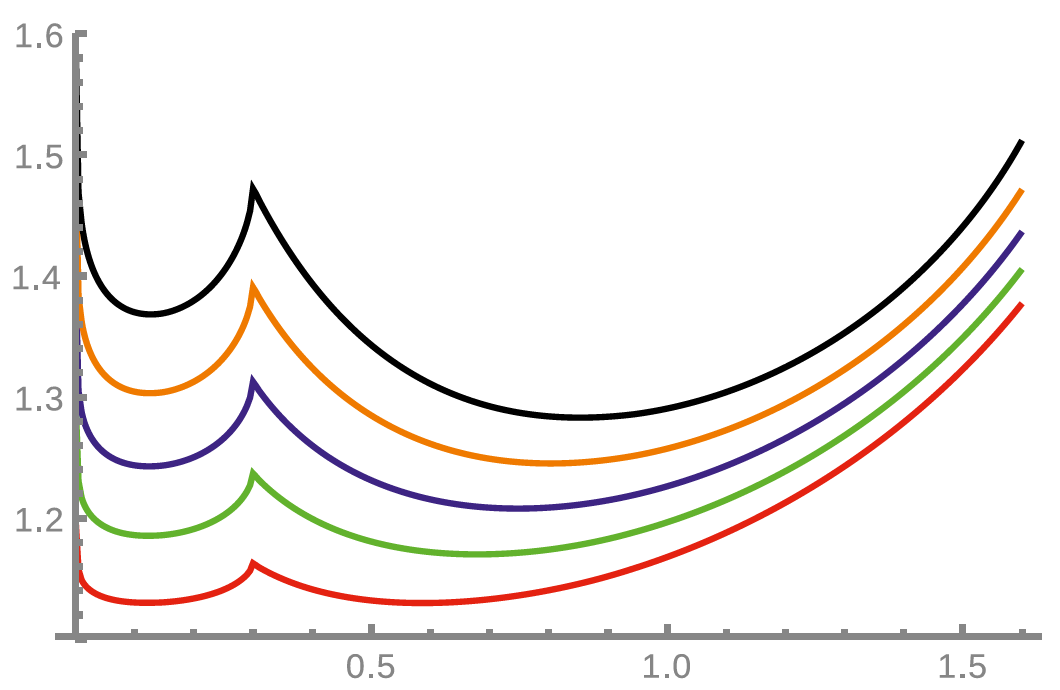
\includegraphics[scale = .25]{plot/3.png}
    \end{minipage}  
    \begin{minipage}[r]{.5\textwidth}
      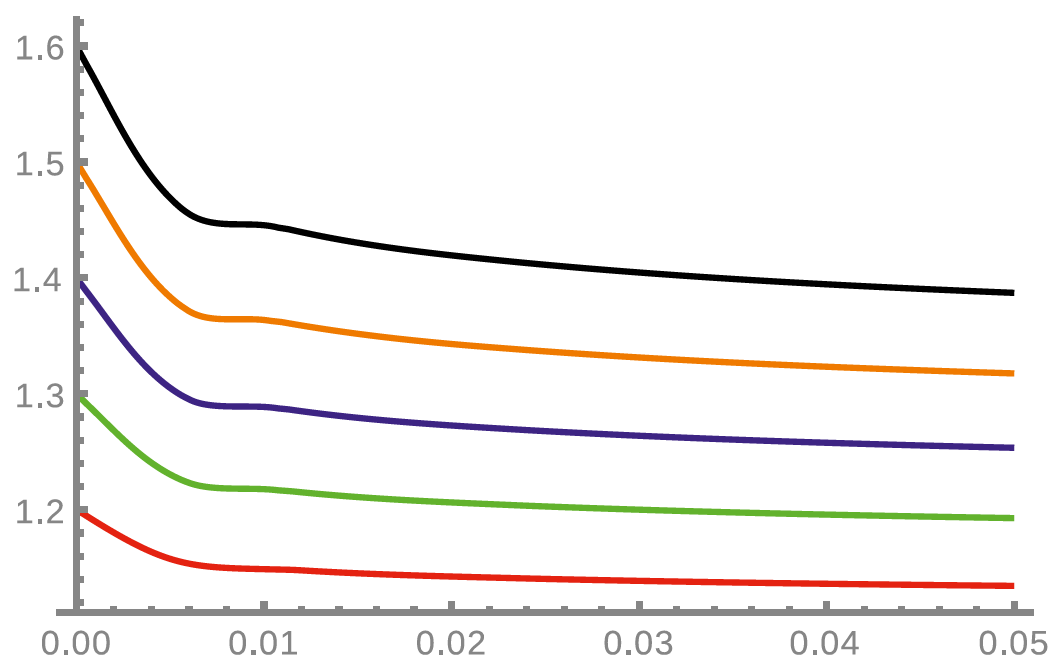
\includegraphics[scale = .25]{plot/4.png}
    \end{minipage} 
    \caption{
        Graphs of solutions to the differential equation $\leftindex[I]^C {D^{0.28}}y(t) = \sqrt{|0.3-t|} \sin(3y(t))+ 0.3t^3$
        with initial conditions $y(0) = 1.2$ (red), $y(0) = 1.3$ (green), $y(0) = 1.4$ (blue), $y(0) = 1.5$ (orange)
        and $y(0) = 1.6$ (black), plotted over the interval $[0, 1.6]$ (left) and zoom of this picture to the interval
        $[0, 0.05]$ (right). It can be observed that the graphs never meet or cross each other.
    } 
\end{figure*}

\newpage
\subsection{Linear Fractional Differential Equations (LFDE)}
A linear FDE is an equation of form
\[
    \left(\leftindex[I]^C {D^{\alpha_m}} + a_{m-1}(t)\leftindex[I]^C {D^{\alpha_{m-1}}} + \dots + a_{1}(t)\leftindex[I]^C {D^{\alpha_{1}}} + a_{1}(t) \right) y(t) = f(t)
\]
With the conditions:
\[
    y^{(k)}(0) = \beta_k \quad,\quad k = 0,1,2,\dots,m-1
\]
\begin{theorem}[Existence And Uniqueness Of LFDE]
    If $f(t)$ is bounded on $(0, T)$ and $a_{k}(t)$ , $k = {0, 1, \dots , m-1}$ 
    are continuous functions on $[0, T]$, the equation has a unique solution.
\end{theorem}
In the particular case where the given differential equation is linear, it is often possible
to write up the solutions in closed form.
\begin{example}
    Show that 
    \[
        y(t) = \frac{1}{\Gamma(\alpha)}\int_{0}^{t} (t-s)^{\alpha-1}f(s) \hquad ds
    \]
    Solves the IVP 
    \[
        \begin{cases}
            \leftindex[I]^C {D^{\alpha}} y(t) = f(t)    \quad&,\quad m-1<\alpha<m
            \\
            I.C \Longrightarrow y^{(k)}(0) = 0 \quad&,\quad k = 0,1,2,\dots,m-1
        \end{cases}
    \]
    \textit{ \textbf{Sol.} } We apply the Laplace transform
        \begin{align*}
            \mathcal{L}\left[\leftindex[I]^C {D^{\alpha}} y(t)\right] &= \mathcal{L}[f(t)]
            \\
            s^{\alpha} Y(s) &= F(s)
            \\
            Y(s) &= s^{-\alpha}F(s)
            \\
            \mathcal{L}[y(t)] &= \mathcal{L}\left[I^{\alpha}f(t)\right]
            \\
            y(t) &= I^{\alpha}f(t) = \frac{1}{\Gamma(\alpha)}\int_{0}^{t} (t-s)^{\alpha-1}f(s) \hquad ds
        \end{align*}
\end{example}
\begin{enrichment*}{Laplace of Mittag Leffler Function }
    \[
        \mathcal{L}\left[t^{\beta-1} E_{\alpha,\beta}(\lambda t^\alpha)\right] = \frac{s^{\alpha - \beta}}{s^{\alpha}-\lambda}
    \]
\end{enrichment*}
\begin{example}
    Show that 
    \[
        y(t) = \sum_{k=0}^{m-1} \beta_k t^{k} E_{\alpha,k+1}(\lambda t^\alpha)
    \]
    Solves the IVP 
    \[
        \begin{cases}
            \leftindex[I]^C {D^{\alpha}} y(t) = \lambda y(t)    \quad&,\quad m-1<\alpha<m
            \\
            I.C \Longrightarrow y^{(k)}(0) = \beta_k \quad&,\quad k = 0,1,2,\dots,m-1
        \end{cases}
    \]
    \textit{ \textbf{Sol.} } We apply the Laplace transform
        \begin{align*}
            \mathcal{L}\left[\leftindex[I]^C {D^{\alpha}} y(t)\right] &= \lambda \mathcal{L}[y(t)]
            \\
            s^{\alpha} Y(s) - \sum_{k=0}^{m-1} s^{\alpha-k-1} y^{(k)}(0) &= \lambda Y(s)
            \\
            Y(s) &= \sum_{k=0}^{m-1} \frac{s^{\alpha-k-1}}{s^{\alpha}-\lambda} \beta_k
            \\
            \mathcal{L}[y(t)] &= \sum_{k=0}^{m-1} \mathcal{L}\left[\beta_k t^{k} E_{\alpha,k+1}(\lambda t^\alpha)\right]
            \\
            \mathcal{L}[y(t)] &= \mathcal{L}\left[\sum_{k=0}^{m-1} \beta_k t^{k} E_{\alpha,k+1}(\lambda t^\alpha)\right]
            \\
            y(t) &= \sum_{k=0}^{m-1} \beta_k t^{k} E_{\alpha,k+1}(\lambda t^\alpha)
        \end{align*}
\end{example}
In example (6.1.4) if we take special case when $m-1 = 0$ and for $\lambda = -1$. 
\[
    y(t) = \beta_0 E_{\alpha,1}(-t^\alpha)
\]
The cases $\alpha = 1$ and $\alpha = 2$
reduce to the well known statements that are the exponential function $E_{1,1}(-t) = e^{-t}$ and
the cosine $E_{2,1}(-t^2) = cos(t)$ solve the given first and second order IVPs.

This observation indicates that the solutions to the general problem of order $\alpha$ 
decay in a monotonic way for $\alpha = 1$ and exhibit persistent oscillations for $\alpha = 2$ if $\lambda$ is
a negative real number. 
And the behavior of the solution in the cases $1 < \alpha < 2$ and $0 < \alpha < 1$. 
The associated results are illustrated in Figure 2
\begin{figure*}[h]
    \begin{minipage}[l]{.5\textwidth}
      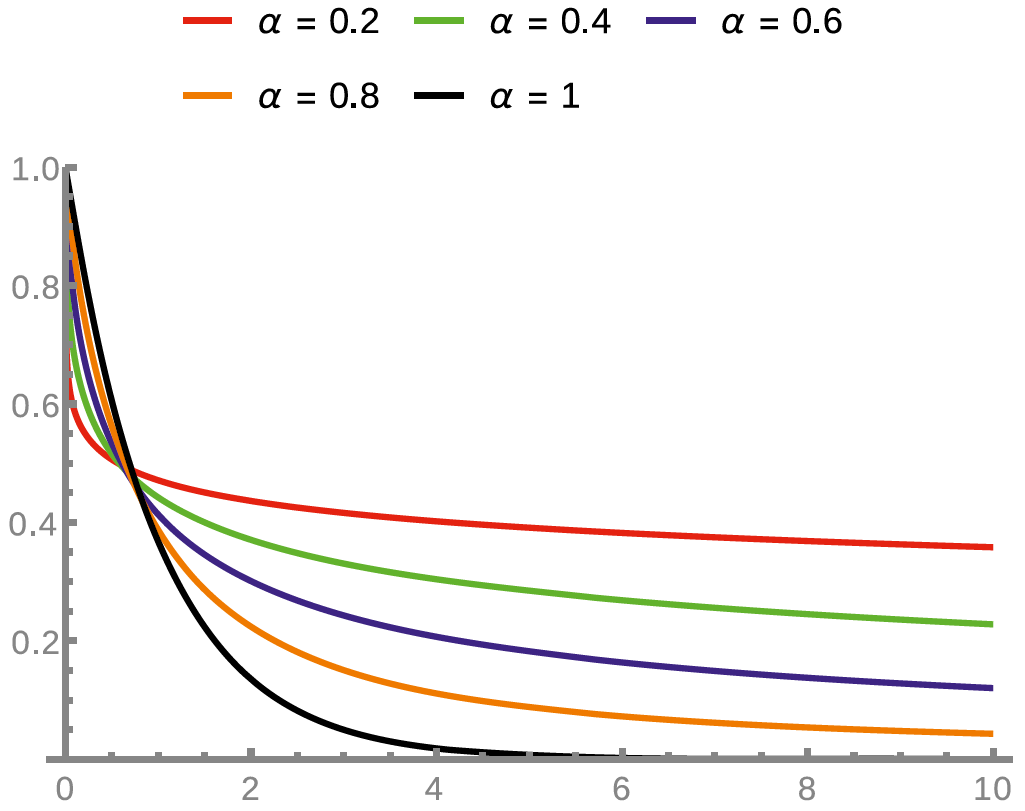
\includegraphics[scale = .25]{plot/1.png}
    \end{minipage}  
    \begin{minipage}[r]{.5\textwidth}
      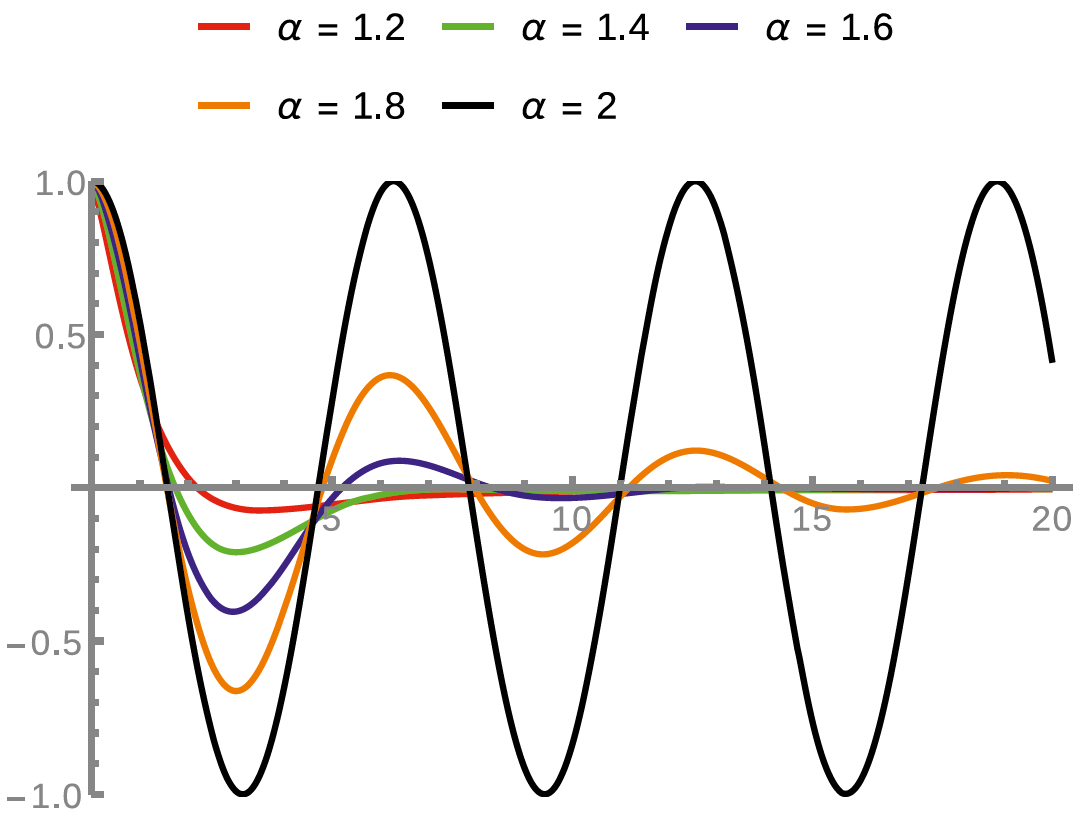
\includegraphics[scale = .25]{plot/2.png}
    \end{minipage} 
    \caption{Plots of $y(t) = E_{\alpha}(-t^\alpha)$ for various $\alpha \in (0, 1]$ (left) and $\alpha \in (1, 2]$ (right).} 
\end{figure*}

\begin{example}
    Show that 
    \[
        y(t) = \beta + t^{\alpha} \sum_{n=0}^{\infty} \frac{f^{(n)}(0)}{\Gamma(n+\alpha+1)}t^n
    \]
    Solves the IVP 
    \[
        \begin{cases}
            \leftindex[I]^C {D^{\alpha}} y(t) = f(t)    \quad,\quad 0<\alpha<1
            \\
            I.C \Longrightarrow y(0) = \beta
        \end{cases}
    \]
    \textit{ \textbf{Sol.} } We expand $f(t)$ using Taylor expansion and apply the Laplace transform
        \begin{align*}
            \mathcal{L}[\leftindex[I]^C {D^{\alpha}} y(t)] &= \mathcal{L}[f(t)]
            \\
            s^{\alpha} Y(s) - \beta s^{\alpha-1} &= \mathcal{L}\left[\sum_{n=0}^{\infty} \frac{f^{(n)}(0)}{\Gamma(n+1)}t^n\right]
            \\
            Y(s) &= \frac{\beta}{s} + \sum_{n=0}^{\infty} \frac{f^{(n)}(0)}{\Gamma(n+1)}\frac{1}{s^{\alpha}}\mathcal{L}[t^n]
            \\
            \mathcal{L}[y(t)] &= \mathcal{L}[\beta] + \sum_{n=0}^{\infty} \frac{f^{(n)}(0)}{\Gamma(n+1)}\frac{1}{s^{\alpha}}\frac{\Gamma(n+1)}{s^{n+1}}
            \\
            \mathcal{L}[y(t)] &= \mathcal{L}[\beta] + \sum_{n=0}^{\infty} f^{(n)}(0) \frac{1}{s^{n+\alpha+1}}
            \\
            \mathcal{L}[y(t)] &= \mathcal{L}[\beta] + \sum_{n=0}^{\infty} f^{(n)}(0) \mathcal{L}\left[\frac{t^{n+\alpha}}{\Gamma(n+\alpha+1)}\right]
            \\
            y(t) &= \beta + t^{\alpha} \sum_{n=0}^{\infty} \frac{f^{(n)}(0)}{\Gamma(n+\alpha+1)}t^n
        \end{align*}
\end{example}
% \newpage
\begin{example}
    Solve the in-homogeneous IVP 
    \[
        \begin{cases}
            \leftindex[I]^C {D^{\alpha}} y(t) = \lambda y(t) + Q(t)   \quad&,\quad m-1<\alpha<m
            \\
            I.C \Longrightarrow y^{(k)}(0) = \beta_k \quad&,\quad k = 0,1,2,\dots,m-1
        \end{cases}
    \]
    Where $Q \in C[0, h]$ is a given function 

    \textit{ \textbf{Sol.} } As we did previously we expand $Q(t)$ using Taylor expansion and apply the Laplace transform
    \begin{align*}
        \mathcal{L}\left[\leftindex[I]^C {D^{\alpha}} y(t)\right] &= \lambda \mathcal{L}[y(t)] + \mathcal{L}\left[\sum_{n=0}^{\infty} \frac{Q^{(n)}(0)}{\Gamma(n+1)}t^n\right]
        \\
        s^{\alpha} Y(s) - \sum_{k=0}^{m-1} s^{\alpha-k-1} y^{(k)}(0) &= \lambda Y(s) + \sum_{n=0}^{\infty} Q^{(n)}(0) s^{-n-1} 
        \\
        Y(s) &= \sum_{k=0}^{m-1} \frac{s^{\alpha-k-1}}{s^{\alpha}-\lambda} \beta_k + \sum_{n=0}^{\infty} Q^{(n)}(0) \frac{s^{-n-1} }{s^{\alpha}-\lambda}
        \\
        \mathcal{L}[y(t)] &= \sum_{k=0}^{m-1} \mathcal{L}\left[\beta_k t^{k} E_{\alpha,k+1}(\lambda t^\alpha)\right] + \sum_{n=0}^{\infty} Q^{(n)}(0) \frac{s^{\alpha-\alpha-n-1} }{s^{\alpha}-\lambda}
        \\
        \mathcal{L}[y(t)] &= \mathcal{L}\left[\sum_{k=0}^{m-1} \beta_k t^{k} E_{\alpha,k+1}(\lambda t^\alpha)\right] + \sum_{n=0}^{\infty} \mathcal{L}\left[Q^{(n)}(0) t^{\alpha+n} E_{\alpha,\alpha+n+1}(\lambda t^\alpha)\right]
        \\
        \mathcal{L}[y(t)] &= \mathcal{L}\left[\sum_{k=0}^{m-1} \beta_k t^{k} E_{\alpha,k+1}(\lambda t^\alpha)\right] + \mathcal{L}\left[\sum_{n=0}^{\infty} Q^{(n)}(0) t^{\alpha+n} E_{\alpha,\alpha+n+1}(\lambda t^\alpha)\right]
        \\
        \tag{6.7} y(t) &= \sum_{k=0}^{m-1} \beta_k t^{k} E_{\alpha,k+1}(\lambda t^\alpha) + \sum_{n=0}^{\infty} Q^{(n)}(0) t^{\alpha+n} E_{\alpha,\alpha+n+1}(\lambda t^\alpha)
        \intertext{Using Mittag Leffler function recursion relation $\displaystyle E_{\alpha,\alpha+\beta}(z) = \frac{1}{z}\left[E_{\alpha,\beta}(z) - \frac{1}{\Gamma(\beta)}\right]$}
        &= \sum_{k=0}^{m-1} \beta_k t^{k} E_{\alpha,k+1}(\lambda t^\alpha) + \sum_{n=0}^{\infty} Q^{(n)}(0) t^{\alpha+n} \frac{1}{\lambda t^\alpha}\left[E_{\alpha,n+1}(z) - \frac{1}{\Gamma(n+1)}\right]
        \\
        &= \sum_{k=0}^{m-1} \beta_k t^{k} E_{\alpha,k+1}(\lambda t^\alpha) + \frac{1}{\lambda}\sum_{n=0}^{\infty} Q^{(n)}(0) t^{n}E_{\alpha,n+1}(z) - \frac{Q(t)}{\lambda}
        \setcounter{equation}{7}
    \end{align*}
Another way using the superposition principle
\begin{enrichment*}{The Superposition Principle}
    The solution of the in-homogeneous equation can be written as the 
    sum of the solution of the homogeneous equation, and a particular 
    solution of the in-homogeneous equation.
\end{enrichment*}
We can break the problem into the following two problems
\[
    \begin{cases}
        \leftindex[I]^C {D^{\alpha}} y_h(t) = \lambda y_h(t)  \quad&,\quad m-1<\alpha<m
        \\
        I.C \Longrightarrow y_h^{(k)}(0) = \beta_k \quad&,\quad k = 0,1,2,\dots,m-1
    \end{cases}
\]
\[
    \begin{cases}
        \leftindex[I]^C {D^{\alpha}} y_p(t) = \lambda y_p(t) + Q(t)   \quad&,\quad m-1<\alpha<m
        \\
        I.C \Longrightarrow y_p^{(k)}(0) = 0 \quad&,\quad k = 0,1,2,\dots,m-1
    \end{cases}
\]
Where $y = y_h + y_p$ solves the original problem.
From example (6.3.2) we got that
\[
    y_h(t) = \sum_{k=0}^{m-1} \beta_k t^{k} E_{\alpha,k+1}(\lambda t^\alpha)
\]
Now for the second problem take Laplace Transform for it 
\begin{align*}
    \mathcal{L}\left[\leftindex[I]^C {D^{\alpha}} y_p(t)\right] &= \lambda \mathcal{L}[y_p(t)] + \mathcal{L}\left[\sum_{n=0}^{\infty} \frac{Q^{(n)}(0)}{\Gamma(n+1)}t^n\right]
    \\
    s^{\alpha} Y_p(s) &= \lambda Y_p(s) + \sum_{n=0}^{\infty} Q^{(n)}(0) s^{-n-1} 
    \\
    Y_p(s) &= \sum_{n=0}^{\infty} Q^{(n)}(0) \frac{s^{-n-1} }{s^{\alpha}-\lambda} = \sum_{n=0}^{\infty} Q^{(n)}(0) \frac{s^{\alpha-\alpha-n-1} }{s^{\alpha}-\lambda}
    \\
    \mathcal{L}[y_p(t)] &= \sum_{n=0}^{\infty} \mathcal{L}\left[Q^{(n)}(0) t^{\alpha+n} E_{\alpha,\alpha+n+1}(\lambda t^\alpha)\right]
    \\
    \mathcal{L}[y_p(t)] &= \mathcal{L}\left[\sum_{n=0}^{\infty} Q^{(n)}(0) t^{\alpha+n} E_{\alpha,\alpha+n+1}(\lambda t^\alpha)\right]
    \\
    y_p(t) &= \sum_{n=0}^{\infty} Q^{(n)}(0) t^{\alpha+n} E_{\alpha,\alpha+n+1}(\lambda t^\alpha)
\end{align*}
Adding $y_h + y_p$ we get the result (6.7)
\end{example}
\begin{enrichment*}{Duhamel's Principle}
    If one can solve an IVP for a homogeneous linear differential equation then an in-homogeneous linear differential equation can be solved as well.
\end{enrichment*} 
\newpage
\subsection{Nonlinear Equations}
Now we will discuss One of the methods to solve Nonlinear FDE which is The Adomian Decomposition Method

The Adomian method applied to the ordinary and partial differential equations of integer order was extended 
also to the case of FDE.
\subsubsection{The Adomian Decomposition Method (ADM)}
Before we talk about how to solve FDE using ADM let us first see how it work 

Consider the problem
\begin{equation}
    \begin{cases}
        \displaystyle \pdv{u(x,t)}{t} + L(u(x,t)) + N(u(x,y)) = g(x,t)
        \\
        I.C \Longrightarrow \displaystyle u(x,0) = \phi(x)
    \end{cases}
\end{equation}
This is nonlinear partial differential equation of integer order where $L(u(x,t))$ is the linear part and $N(u(x,t))$ is the non-linear part
We will discuss it's solution by ADM
\\
Now, Integrate (6.8) from $0 \to t$
\begin{equation}
    u(x,t) = \phi(x) - \int_{0}^{t} L(u(x,s)) \hquad ds  - \int_{0}^{t} N(u(x,s)) \hquad ds  + \int_{0}^{t} g(x,s) \hquad ds
\end{equation}
Set
\begin{equation}
    u(x,t) = \sum_{n=0}^{\infty} u_n(x,y)
\end{equation}
\begin{equation}
    N(u(x,t)) = \sum_{n=0}^{\infty} A_n(x,y)
\end{equation}
Where $A_0,A_1,A_2,\dots$ are \textbf{Adomian Polynomials} defined as:
\[
    A_n(x,y) = \frac{1}{n!} \dv[n]{}{\lambda} \left( N \left( \sum_{j=0}^{n}\lambda^j u_j \right) \right)
\]
Substitute equations (6.10),(6.11) into (6.9) we get
\begin{equation*}
    u(x,y) = \sum_{n=0}^{\infty}u_n(x,t) = \phi(x) + \int_0^t g(x,s) \hquad ds - \int_0^t L \left(\sum_{n=0}^{\infty}u_n(z,t)\right)  - \int_0^t \sum_{n=0}^{\infty}A_n(x,s) \hquad ds
\end{equation*}
Now,
\begin{align*}
    u_0 & = \phi(x) + \int_0^t g(x,s) \hquad ds                 \\
    u_1 & = -\int_0^t L(u_0) \hquad ds - \int_0^t A_0 \hquad ds         \\
    u_2 & = -\int_0^t L(u_1) \hquad ds - \int_0^t A_1 \hquad ds         \\
    \vdots                                               \\
    u_n & = -\int_0^t L(u_{n-1}) \hquad ds - \int_0^t A_{n-1} \hquad ds
\end{align*}
\[
    \therefore u(x,t) = \sum_{n=0}^{\infty} u_n(x,y) = u_0 + u_1 + u_2 + \dots
\]
This will get the solution for the problem (6.8)
\newpage
Note that The Adomian Decomposition Method (ADM)
is a numerical technique used to approximate solutions
of differential equations.
Whether ADM converges or diverges depends on the
specific problem and how it is applied.
The convergence and divergence of ADM can be
influenced by several factors, including the
complexity of the problem, the choice of the
decomposition functions, and the behavior of
the nonlinear terms in the differential equation.

\begin{example}
    Solve the nonlinear differential equation using ADM
    \begin{equation}
        \begin{cases}
            \displaystyle \frac{\partial u(x,t)}{\partial t} = x^2 - \frac{1}{4}\left( \frac{\partial u(x,t)}{\partial x} \right)^2
            \\
            I.C \Longrightarrow \displaystyle u(x,0) = 0
        \end{cases}
    \end{equation}
    \textit{ \textbf{Sol.} } Set
    \begin{align*}
        u(x,t) & = \sum_{n=0}^{\infty} u_n(x,t)
        \\
        N(u)   & = \sum_{n=0}^{\infty} A_n(x,t)
    \end{align*}
    Where $N(u)$ represents the nonlinear form of $u$ 
    
    In our case in equation (6.12) $\displaystyle N(u) = \left(\frac{\partial u}{\partial x}\right)^2$
    \begin{align*}
        A_n(x,t) & = \left[\frac{1}{n!} \frac{d^n}{d \lambda^n} N\left(\sum_{i=0}^{n}  \lambda^i u_i(x,t)\right)\right]_{\lambda = 0}
        \\
        A_n(x,t) & = \left[\frac{1}{n!} \frac{d^n}{d \lambda^n} \left(\sum_{i=0}^{n}  \lambda^i \frac{\partial u_i(x,t)}{\partial x}\right)^2\right]_{\lambda = 0}
    \end{align*}
    Integrating equation (6.12) from $0 \to t$
    \[
        u(x,t) = \sum_{n=0}^{\infty} u_n(x,t)  = x^2t - \frac{1}{4} \int_{0}^{t}\sum_{n=0}^{\infty} A_n(x,\theta) \hquad d\theta
    \]
    Now we get $A_0$,$A_1$,$A_2,\dots$
    \begin{align*}
        A_0(x,\theta) & = \left[\sum_{i=0}^{0}  \lambda^i \frac{\partial u_i(x,\theta)}{\partial x}^2\right]_{\lambda = 0} = \left(\frac{\partial u_0(x,\theta)}{\partial x}\right)^2
        \\
        A_1(x,\theta) & = \left[\frac{d}{d \lambda} \left(\sum_{i=0}^{1}  \lambda^i \frac{\partial u_i(x,\theta)}{\partial x}\right)^2\right]_{\lambda = 0}
        \\
                      & = \left[\frac{d}{d \lambda} \left(\frac{\partial u_0(x,\theta)}{\partial x} + \lambda \frac{\partial u_1(x,\theta)}{\partial x}\right)^2\right]_{\lambda = 0}
        \\
                      & =2\left[\left(\frac{\partial u_0(x,\theta)}{\partial x} + \lambda \frac{\partial u_1(x,\theta)}{\partial x}\right)\frac{\partial u_1(x,\theta)}{\partial x}\right]_{\lambda = 0} = 2\frac{\partial u_0(x,\theta)}{\partial x} \frac{\partial u_1(x,\theta)}{\partial x}
        \\
        A_2(x,\theta) & =\left[\frac{1}{2!} \frac{d^2}{d \lambda^2} \left(\sum_{i=0}^{2}  \lambda^i \frac{\partial u_i(x,\theta)}{\partial x}\right)^2\right]_{\lambda = 0}
        \\
                      & = \left[\frac{1}{2} \frac{d^2}{d \lambda^2} \left(\frac{\partial u_0(x,\theta)}{\partial x} + \lambda \frac{\partial u_1(x,\theta)}{\partial x} + \lambda^2 \frac{\partial u_2(x,\theta)}{\partial x}\right)^2\right]_{\lambda = 0}
        \\
                      & = \left(\frac{\partial u_1(x,\theta)}{\partial x}\right)^2 + 2 \left(\frac{\partial u_0(x,\theta)}{\partial x}\frac{\partial u_2(x,\theta)}{\partial x}\right)
        \\
        A_3(x,\theta) & = 2\frac{\partial u_1(x,\theta)}{\partial x}\frac{\partial u_2(x,\theta)}{\partial x} + 2\frac{\partial u_0(x,\theta)}{\partial x} \frac{\partial u_3(x,\theta)}{\partial x}
    \end{align*}
    Now because
    \[
        u_0 + u_1 + u_2 + \dots = u(x,t) = x^2t - \frac{1}{4}\int_{0}^{t}[A_0+A_1+A_2+\dots] \hquad d\theta
    \]
    Then
    \begin{align*}
        u_0 & = x^2t
        \\
        u_1 & = -\frac{1}{4}\int_{0}^{t}A_0d\theta = -\frac{1}{4}\int_{0}^{t}\left(\frac{\partial u_0(x,\theta)}{\partial x}\right)^2 = -\int_{0}^{t} x^2 \theta^2 d\theta = \frac{-1}{3}x^2t^3
        \\
        u_2 & = \frac{2}{15} x^2t^5
        \\
        u_3 &= \frac{-17}{315} x^2t^7 
        \\
        \vdots
    \end{align*}
    \[
        u(x,t) = x^2 \left[t-\frac{1}{3}t^3 + \frac{2}{15} t^5 - \frac{17}{315} t^7 \dots\right] = x^2 \tanh(t)
    \]
\end{example}
\begin{figure}[b]
    \begin{enrichment}{George Adomian}{Chars/adom.jpg}{2.4}{.8}{.17}
        George Adomian (March 21, 1922 – June 17, 1996)
        was an American mathematician of Armenian descent
        who developed the Adomian decomposition method (ADM)
        for solving nonlinear differential equations,
        both ordinary and partial.
        The method is explained among other places
        in his book \textit{\textbf{"Solving Frontier Problems in Physics:
                The Decomposition Method"}}.
        He was a faculty member at the University of Georgia
        (UGA) from 1966 through 1989. While at UGA,
        he started the Center for Applied Mathematics.
        Adomian was also an aerospace engineer.
    \end{enrichment}
\end{figure}
\newpage
\subsubsection{Decomposition Of Nonlinear FDE}
We consider the following nonlinear FDE 
\begin{equation}
    \begin{cases}
        \displaystyle \leftindex[I]^C {D^{\alpha}} y(t) + L(y(t)) + N(y(t)) = f(t)
        \\
        I.C \Longrightarrow \displaystyle y^{(k)}(0) = \beta_k \quad,\quad k=0,1,2,\dots,m-1 
    \end{cases}
\end{equation}
We apply the Laplace Transform to the equation
\[
    \mathcal{L}[\leftindex[I]^C {D^{\alpha}} y(t)] = s^{\alpha} Y(s) - \sum_{k=0}^{m-1} s^{\alpha-k-1} y^{(k)}(0)
\]
We use the following decomposition of $y(t)$
\[
    y(t) = \sum_{n=0}^{\infty} y_n(t)
\]
And 
\[
    N(y(t)) = \sum_{n=0}^{\infty} A_n
\]
Where $A_n$ are Adomian polynomials

The equation (6.13) become 
\[
    \mathcal{L}\left[\sum_{n=0}^{\infty} y_n(t)\right] = \sum_{k=0}^{m-1} \frac{\beta_k}{s^{k+1}} - \frac{1}{s^{\alpha}} \mathcal{L}\left[L\left(\sum_{n=0}^{\infty} y_n(t)\right)\right] - \frac{1}{s^{\alpha}}\mathcal{L}\left[\sum_{n=0}^{\infty} A_n\right] + \frac{1}{s^{\alpha}}\mathcal{L}\left[f(t)\right]
\]
Now we can get 
\begin{align*}
    Y_0 &= \mathcal{L}\left[y_0\right] = \sum_{k=0}^{m-1} \frac{\beta_k}{s^{k+1}} + \frac{1}{s^{\alpha}}\mathcal{L}\left[f(t)\right]
    \\
    Y_1 &= \mathcal{L}\left[y_1\right] = - \frac{1}{s^{\alpha}} \mathcal{L}\left[L\left(y_0(t)\right)\right] - \frac{1}{s^{\alpha}}\mathcal{L}\left[ A_0\right]
    \\
    Y_2 &= \mathcal{L}\left[y_2\right] = - \frac{1}{s^{\alpha}} \mathcal{L}\left[L\left(y_1(t)\right)\right] - \frac{1}{s^{\alpha}}\mathcal{L}\left[ A_1\right]
    \\
    \vdots
    \\
    Y_n &= \mathcal{L}\left[y_n\right] = - \frac{1}{s^{\alpha}} \mathcal{L}\left[L\left(y_{n-1}(t)\right)\right] - \frac{1}{s^{\alpha}}\mathcal{L}\left[ A_{n-1}\right]
\end{align*}
\begin{example}
    Solve the nonlinear FDE using the Adomian decomposition method
    \[
        \begin{cases}
            \displaystyle \leftindex[I]^C {D^{\alpha}} y(t) = t + y^2 \quad,\quad 1<\alpha \leq 2
            \\
            I.C \Longrightarrow \displaystyle y(0) = 0 \quad,\quad y^{(1)}(0) = 1
        \end{cases}
    \]
    \textit{ \textbf{Sol.} } In order to solve the equation we apply the Laplace transform
    \begin{align*}
        \mathcal{L}\left[\leftindex[I]^C {D^{\alpha}} y(t)\right] &= \mathcal{L}\left[t + y^2\right]
        \\
        s^{\alpha} Y(s) - s^{\alpha-1}y(0) - s^{\alpha-2} y^{(1)}(0) &= \mathcal{L}\left[t + y^2\right]
        \\
        s^{\alpha} Y(s) - s^{\alpha-2} &= \mathcal{L}\left[t + y^2\right]
    \end{align*}
    So that, for the decomposition
    \[
        y(t) = \sum_{n=0}^{\infty} y_n(t)
    \]
    We obtain
    \[
        Y(s) = \sum_{n=0}^{\infty} Y_n(s) \quad , \quad t+y^2 = \sum_{n=0}^{\infty} A_n
    \]
    The Adomian polynomials $A_n$ are 
    \[
        A_0 = t + y_0^2 \quad,\quad A_1 = 2y_0y_1 \quad,\quad A_2 = y_1^2 + 2y_0y_2 \quad,\quad A_2 = 2y_1y_2 + 2y_0y_3 \quad,\dots
    \]
    \[
        Y_0 = \frac{1}{s^2} \quad\Longrightarrow\quad y_0 = t \quad\Longrightarrow\quad A_0 = t+t^2
    \]
    \[
        Y_1 = \frac{1}{s^\alpha}\mathcal{L}\left[A_0\right] \quad\Longrightarrow\quad y_1 = \frac{t^{\alpha+1}}{\Gamma(\alpha+2)} + 2\frac{t^{\alpha+2}}{\Gamma(\alpha+3)} \quad\Longrightarrow\quad A_1 = 2y_0y_1
    \]
    And so on 
    \[
        y(t) = y_0 + y_1 + y_2 + \dots
    \]
\end{example}


\subsection{Fractional Systems of Differential Equations}
Solving System of FDE is not very different from solving single FDE 
there are Linear Systems which can be solved using Laplace Transform 
and we will show example of them and there are Nonlinear Systems
which can be solved by Method of Successive Approximations and
The Adomian Decomposition Method

\begin{example}
    Solve the system of FDE
    \[
        \begin{cases}
            \displaystyle \leftindex[I]^C {D^{\alpha}} x(t) = \leftindex[I]^C {D^{\beta}} y(t) + 1  \quad,\quad 0<\alpha<1
            \\
            \displaystyle \leftindex[I]^C {D^{\beta}} y(t) = 2\leftindex[I]^C {D^{\alpha}} x(t) - 1 \quad,\quad 0<\beta<1
            \\
            I.C \Longrightarrow x(0) = 1 \quad,\quad y(0) = 1
        \end{cases}
    \]
    \textit{ \textbf{Sol.} } We apply the Laplace Transform method
    \[
        \begin{cases}
            \displaystyle \mathcal{L}\left[\leftindex[I]^C {D^{\alpha}} x(t) \right]= \mathcal{L}\left[\leftindex[I]^C {D^{\beta}} y(t)\right] + \mathcal{L}\left[1\right]
            \\
            \displaystyle \mathcal{L}\left[\leftindex[I]^C {D^{\beta}} y(t) \right]= 2\mathcal{L}\left[\leftindex[I]^C {D^{\alpha}} x(t)\right] - \mathcal{L}\left[1\right]
        \end{cases}
    \]
    We obtain the system
    \[
        \begin{cases}
            \displaystyle s^\alpha X(s) - s^{\alpha-1} = s^\beta Y(s) - s^{\beta-1} + \frac{1}{s}
            \\
            \displaystyle s^\beta Y(s) - s^{\beta-1} = 2s^\alpha X(s) - 2s^{\alpha-1} - \frac{1}{s}
        \end{cases}
    \]
    With the solution:
    \[
        \begin{cases}
            \displaystyle X(s) = \frac{1}{s}
            \\\\
            \displaystyle Y(s) = \frac{1}{s} - \frac{1}{s^{\beta+1}}
        \end{cases}
    \]
    Take the Laplace inverse we get the solution for the original system
    \[
        \begin{cases}
            \displaystyle x(t) = 1 
            \\\\
            \displaystyle y(t) = 1 - \frac{t^{\beta}}{\Gamma(\beta+1)}
        \end{cases}
    \]
\end{example}